%% Why is this interesting?

%\comment{Motivation of paper: improve tracking control through IDM, enable model predictive control with contact for planning}
%Tracking need precise IDM model.
A key challenge for torque-controlled humanoid robots is to accurately
estimate their dynamics in presence of contacts, e.g.,
during manipulation in clutter
\cite{Jain2013clutter}, whole-body movements
\cite{Handbook2008legged} or ground contacts in locomotion~\cite{Calandra2014}.
Analytic dynamics models suffer from inaccurate parameter estimation, unmodeled dynamics (e.g., friction, couplings, elasticities) and noisy sensor measurements.
With contacts the problem is even more challenging due to discontinuities and additional non-linearities, which are difficult to model or estimate.
%One particular reason for this challenge is that
%contacts cause non-linearities in the system dynamics, which
%are difficult to model analytically or estimate. 
Moreover, if contact locations are not fixed a priori or known with sufficient precision, small errors in the localization of the external force can substantially deteriorate the inverse dynamics computation~\cite{DelPrete2012}.
%Additionally, analytic models suffer from inaccurate dynamic parameters, unmodeled dynamics (e.g., friction, couplings, elasticities) and noisy sensor measurements.
%play in the joints => can be solved kinematically

Nevertheless, many modern control strategies like inverse dynamics control~\cite{Erez2012}, computed torque control~\cite{Siciliano2009} or model predictive control~\cite{Naveau2014} rely on accurate 
% too risky: there are techniques in NMPC that do not need this 
%(or even differentiable) dynamics models.
dynamic models.
With inaccurate dynamics models they can produce suboptimal policies by not taking external forces  into account, which are caused by contacts.

\begin{wrapfigure}{r}{0.3\columnwidth}
%\begin{figure}[t]
	%\vspace{-10pt}
	\centering
	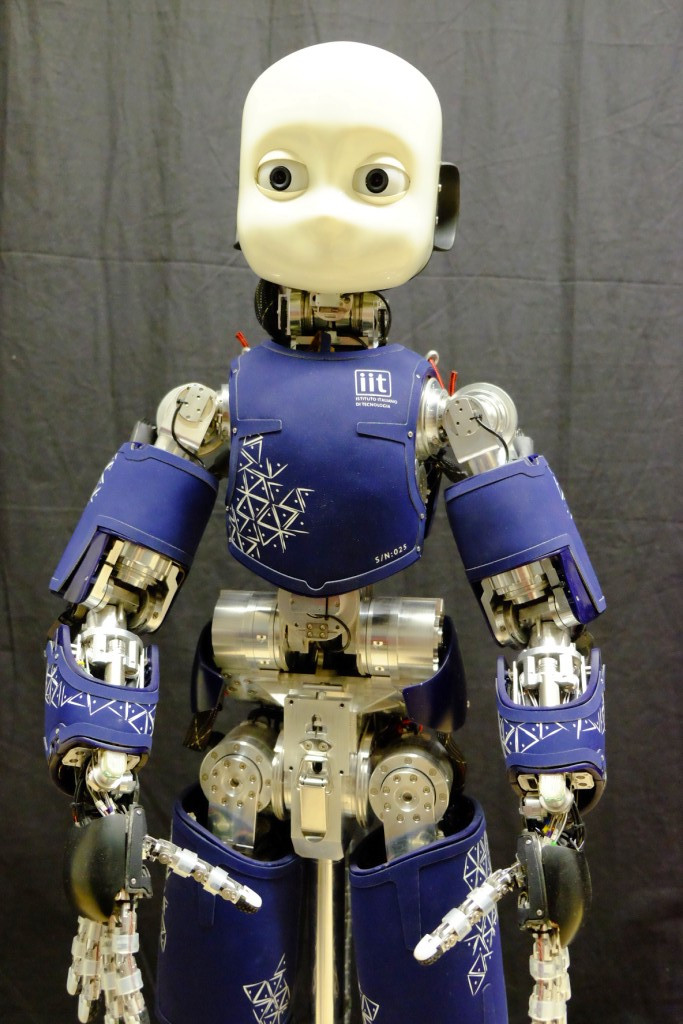
\includegraphics[width=.99\linewidth]{robertoICRA/fig/iCubDarmstadt01}
	\caption{The humanoid robot \robot{} used in the experiments.}
	\label{fig:icub}
	\figspace
%\end{figure}
\end{wrapfigure}

As a first step toward a more informed controller that explicitly considers the effect of contacts, we propose 
%
%
to learn the inverse dynamics model from tactile sensor readings and force-torque sensors. 
%
In contrast to classical techniques based on the identification of dynamics parameters~\cite{Yamane2011calibration,Ogawa2014,traversaro2013inertial},
we propose a fully data-driven machine learning approach based on non-parametric models,
where both the rigid body dynamics as well as the effect of external forces on the
robot structure are learned directly from data collected on the real robot.
%
The proposed model makes use of the raw sensor data and does not require a kinematic/dynamics calibration~\cite{Yamane2011calibration,Ogawa2014,traversaro2013inertial}. 
In particular, it does not need a spatially calibrated model of the skin~\cite{DelPrete2011}.
%
We propose to use a mixtures-of-experts based on Gaussian Processes (GP) to learn the non-linear system dynamics.
Each of these GP experts models a single contact ``type'' and can be learned straightforwardly.
By using a gating network that activates and deactivates the individual GP experts we can switch between contact models and generalize to more complex environments.
% \todo[inline, color=yellow]{I don't think this bit is necessary here...\\
% As ground-truth we use joint-torque sensor measurements,
% and  we compare to a state-of-the-art analytic modeling approach
% that assumes perfect knowledge of the contact location to model external forces.
% Our approach in contrast, uses simply the tactile information to activate the experts.}
% The Gaussian processes are trained with the robot configurations (in joint angles)
% and the force measurements of the joint-torque sensors.
We evaluate our model learning approach on the arm of the \robot{} humanoid robot~\cite{Natale2013} (see \fig\ref{fig:icub}) and compare to a state-of-the-art model-based approach.
The learned inverse dynamics model outperforms the analytic approach and we demonstrate that the learned model can generalize to changing contact locations.
To the best of our knowledge this is the first demonstration of how joint torques can be learned on a humanoid robot equipped with tactile and force/torque sensors in presence of contacts.
%these sensor modalities\todo{What do you mean by "sensor modality"?}. 

%==========

%Both simulation and control techniques need accurate dynamics models to determine joint torques and external forces at different contact locations. For instance, Computed Torque Control needs a precise model to perform\todo{??} \cite{Siciliano2009}, while Model Predictive Control needs also rapid computation, since it has to compute the entire robot dynamics over a receding time horizon at each control step (as in \cite{naveau2014metapod}, within 1--2~$\mu$s).
% \todo[inline]{Besides accuracy and time constraints, a fundamental requirement is
% the capability to handle multiple simultaneous contacts, which poses
% several problems for the computation of inverse robot dynamics and
% trajectory optimization
% \cite{erez2012trajectory}.}


%for instance Model Predictive Control or computed torque control, need 
%To achieve fast, stable and precise performances in tracking of desired torques and regulation of contact forces, control techniques, for instance  
%
%Humanoid robots need to precisely control their interaction forces during contacts with the environment. %, relying on precise dynamics models.
%In case of multiple contacts, such as during manipulation in clutter \cite{Jain2013clutter} and whole-body movements \cite{Handbook2008legged}, an accurate dynamics model is critical to obtain a precise estimation of the joint torques and the external forces at the different contact locations. 
%To synthesize whole-body motions, Model Predictive Control techniques also need to compute the robot dynamics over a receding time horizon \cite{naveau2014metapod}. 
%More in general, many nonlinear control approaches, such as computed torque control, need accurate and fast models to perform \cite{Siciliano2009}.
%
%Besides accuracy, these techniques pose substantially two requirements: first, the capability to rapidly compute the dynamics (as in \cite{naveau2014metapod}, within 1-2 $\mu$s); second, the capability to handle multiple simultaneous contacts.

%\todo[inline]{What approaches are usually used for modeling contacts?
%  Why are they not so good? How do we address this shortcoming in this
%paper? What are the contributions?}


%%--------------------------------------------
%% INDUSTRIAL ROBOTS
%%--------------------------------------------
%
% For industrial manipulators the contact location is usually placed at the end-effector, so it is frequent to consider one single contact and write the equation as:
% %
% \begin{align}\label{eq:tau_onecontact}
% 	\torques = \inertiaMatrix\ddq + \Hmatrix + \jacobian\T_c(\q) \forceNo
% \end{align}
% %
% where notably the term $\epsilon(\q,\dq,\ddq)$ is also neglected. 
% Its effects are usually compensated by robust control design or simply raising the gains in the joint controllers. 
% The external force~$\forceNo$ can be easily measured at the end-effector through dedicated sensors, for example 6-axis force/torque sensors.
% 
% 
% For more complex robots, particularly humanoids, the classical hypothesis of a single and known contact does not hold. 
% Humanoid robots have to navigate in cluttered and evolving environments, which requires the ability to cope with multiple contacts occurring on their whole-body. 
% Contact locations cannot be known or fixed in advance (they are a consequence of the environment and the robot's movement), but they can be predicted or measured by distributed tactile sensors, i.e. skin elements. 
%
%
%%--------------------------------------------

%The knowledge of the robot dynamics is fundamental for controlling the joint torques and planning whole-body dynamics movements. 
%In general, we would like to generate trajectories that are optimal for some specified criterion (minimization of effort, energy, etc.), obtaining desired $[\q^\star,\dq^\star,\ddq^\star]$. If the inverse dynamic is known, then we can use either \eq\ref{eq:tau_nocontact} or \eq\ref{eq:tau_contact} to compute the necessary $\torques$ depending on the contact situation. 
%If the joint to motor torque relationship is known, then we can precompute optimal trajectories or adapt them online very efficiently.
%However, in most of the robots such performance is hard to achieve, for many reasons. For instance, the robot dynamics model is often inaccurate, and it is difficult to estimate the dynamic parameters correctly.
%\textbf{Methods for computing the robot dynamics}: 


%%% must be re-written, shorter
%If identification of industrial robot is relatively easy with exciting trajectories \cite{Pedrocchi2014}, the procedure for floating-base robots such as humanoids is not straightforward. The main issue is the generation of accelerations large enough for the identification while maintaining the robot balance and the control of contacts. The issue was well explained by Yamane in \cite{yamane2011calibration}, which proposed a technique to identify the mass and the local COM of the links in a humanoid robot with fixed feet at the ground and slow joint trajectories. Unable to  identify the inertial parameters, the CAD models were used. Traversaro et al. in \cite{traversaro2013inertial} proposed a technique to identify the inertial parameters based on motor currents, force/torque measurements and robot trajectories, however performed in absence of contacts.
%Ogawa et al. \cite{ogawa2014identification} proposed to identify the base parameters from joint torque sensing and external forces, requiring the knowledge of the contact force and location. They applied it on the humanoid Toro, walking without additional contacts.
%When multiple contacts are exerted on the robot structure in locations other than the classical end-effectors, it is still possible to compute a precise dynamics, but this requires either pervasive joint torque sensing, such as in Toro \cite{ogawa2014identification} or additional sensing (tactile, force/torque) such as in iCub \cite{Ivaldi2011,Fumagalli2012}.


% %Overall, these approaches have three main limits: 1) they are model-based, therefore it is more and more complex to add couplings, elasticity, friction and other nonlinear dynamics; 2) the parameters-identification is data-driven, therefore the performance of the identification strongly depends on the experimental setting (with/without contacts) and the exciting trajectories \cite{Pedrocchi2014}; 3) they deal with contacts under restrictive assumptions.


% An alternative and appealing approach to model-based dynamics computation is to use machine learning methods to learn the dynamics model of a robot~\cite{Nguyen-Tuong2008,Vijayakumar2000}. 
% The clear advantage of learning the inverse dynamics is that we can overcome the limitations of the aforementioned approaches: difficulty in modeling complex nonlinear dynamics, impossibility to generate suitable exciting trajectories, restrictive assumptions regarding contacts and sensors, prior accurate kinematics calibration of the tactile sensors.\todo[inline]{Unclear how learning overcomes these limitations}
% %Several machine learning techniques have been applied to the problem of learning inverse dynamics, for example GP~\cite{???}, LGP~\cite{Nguyen-Tuong2008} and LWPR~\cite{Vijayakumar2000}.
% %The better performance comes from the fact that we can easily learn unmodelled dynamics and the accumulated errors due to the inaccurate dynamics parameters. 
% %For example, in \cite{Nguyen-Tuong2011} a learned dynamics could improve tracking performances in computed torque control for an industrial manipulator.
% Without the need for compensating for inaccurate dynamics parameters and accumulated errors, a learned dynamics model can improve the tracking and control performances of a robot substantially as shown in~\cite{Nguyen-Tuong2011} for an industrial manipulator.

% However, prior works on learning or improving the inverse dynamics model lack a fundamental aspect: the inclusion of multiple contact dynamics in the model.
% There are two main problems.
% First, it is required to switch from a no-contact model to a contact-model, which requires to observe the the system state and to model a discontinuous function~\cite{Toussaint2005}. 
% Second, it is required to switch between different contact models $c_i \in\mathcal{C}$. %and to combine multiple ones simultaneously: that is dealing with a multitude of  $c_i \in\mathcal{C}$.\todo{unclear}

% % In this paper we focus on the latter problem.\todo{more precise!}
% % To the best of our knowledge there are no examples in the literature where inverse dynamics is learned in the case of multiple contacts.
% %%
% %\begin{align}
% %	\torques = \begin{cases}  \torques_\text{IDM}(\q,\dq,\ddq) &\mbox{no contact }  \\
% %	\torques_\text{IDM}(\q,\dq,\ddq, \forceNo, \jacobian_c) & \mbox{contact } \end{cases} \,,
% %\end{align}
% %%
% %which also requires the ability to observe the system state and know in which case we are. 
% %The main issue is to be able to switch between different contact models and to be able to combine different contacts at the same time (\eq\ref{eq:tau_contact}):
% %%
% %\begin{align}
% %	\torques = \begin{cases}  \torques_\text{IDM}(\q,\dq,\ddq) &\mbox{no contact}  \\
% %	\torques_\text{IDM}(\q,\dq,\ddq, \forceNo_1, \jacobian_{c_1}) & \mbox{contact 1}\\
% %	\torques_\text{IDM}(\q,\dq,\ddq, \forceNo_2, \jacobian_{c_2}) & \mbox{contact 2}\\
% %	\torques_\text{IDM}(\q,\dq,\ddq, \forceNo_1, \forceNo_2, \jacobian_{c_1}, \jacobian_{c_2}) & \mbox{contact 1 \& 2} \\
% %	\ldots
% %	\end{cases}
% %\end{align}
% %
% Here, we provide a first formulation to this problem, and we show that it is possible to learn  the inverse dynamics model of the robot subject to no, one or multiple contacts detected by a distributed tactile skin~$\skinInput$. 


% This solution\todo{What solution?} enables a fast and accurate prediction of joint torques in multiple simultaneous contact situations.
% % when the robot is in contact or not with one or multiple simultaneous contacts, detected by distributed tactile elements. 
% The estimation does not rely on dynamic parameters or models, but is completely sensory-based\todo{data driven?}: notably, it makes use of the raw sensory data and does not require a spatially calibrated model of the skin~\cite{DelPrete2011}.
% We carry out our experiments on the humanoid robot \robot{}~\cite{Natale2013}. We show that it is possible to learn the inverse dynamics model with none, one or multiple contacts detected by its tactile skin. 
% We compare our estimation with the ground truth provided by the joint torque sensors in the arm.
% \todo[]{Something stronger than ``compare''?}

% The paper is organized as follows.
% \sec\ref{sec:mgp} formalize the problem statement and presents our technique to learn multiple contacts. 
% \sec\ref{sec:results} report on the experimental results from different experiments carried out on the humanoid robot \robot{} moving in presence of single and multiple contacts.
% \sec\ref{sec:conclusion} discusses the ongoing work and outlines the future goals.

%%
%For example, in~\cite{Ivaldi2011,Fumagalli2012} the authors used the CAD parameters for estimating the robot dynamics; in~\cite{traversaro2013inertial} improved the dynamics model by identifying the inertial parameters.
%Identifying the dynamics parameters, in general, is non-trivial even for industrial manipulators~\cite{Pedrocchi2013}.
%%=>ref paper silvio, paper sere idyn, papr stima dynamic params poli-milano icra2014 su robot industriale
%Second, it is non-trivial to learn the unmodeled dynamics or improve the dynamics model, because of the lack of suitable sensors. 
%For example, in~\cite{Fumagalli2010a} the authors only had access to a proximal force/torque sensor.

%%%
%Machine learning is an appealing alternative to identification and modelling techniques~\cite{Nguyen-Tuong2011}.
%Several methods have been used to learn the inverse dynamics (i.e., $\torques$), for example  GP~\cite{???}, LGP~\cite{Nguyen-Tuong2008} and LWPR~\cite{Vijayakumar2000}.


% Ways to estimate $\sum J F_i$:
% %
% \begin{itemize}
% 	\item Estimate $F_i$: This is hard as it requires costly and precise torque sensors and to project the estimated forces accurately.
% 	\item Estimate the entire $\color{darkgreen}{\sum_{i \in\mathds{C}} {\jacobian_i(\q)}\T \forceNo_i}$ at the joint level: Can be done by using an observer with higher frequency than the controller.
% 	\item Estimate $\color{darkgreen}{\sum_{i \in\mathds{C}} {\jacobian_i(\q)}\T \forceNo_i}$ from the tactile information.
% \end{itemize}
% %


% % Related works
% \subsection{Related work}

% \todo[inline]{Shall we have a Problem setting section and/or background section here?}

% The are multiple challenges when learning the inverse dynamics for a humanoid robot in presence of contacts:
% \begin{itemize}
%   \item Both state\todo{define} and skin are needed to accurately model the contacts since the dynamics depends not only on the joint configuration of the robot (plus velocities and accelerations), but also on the position of the obstruction.
% 	The state alone is high dimensional, typically in the range of 30 to 50 joints plus, the corresponding velocities and accelerations. 
% 	Additionally, the number of skin sensors alone can be on the order of hundreds or thousands.
% 	Hence, the resulting regression task\todo{what regression task?} is extremely high-dimensional. 
%   \item When creating dynamics models from real measurements we notice how the amount of sensor noise during an impact with an obstruction is substantially higher than the regular sensor noise. 
% 	This is due to the internal dynamics of the sensor and is on some degree inevitable. 
% 	\fixme{For this reason, an accurate model should consider the presence of heteroscedastic noise which is not constant.}
% 	\fixme{variable input GP}
%   \item Impact with obstructions also introduce discontinuities in terms of joint position, velocity, acceleration and torques.
% 	\fixme{These discontinuities cannot be }
% \end{itemize}

	
% \todo[inline]{Not sure what the next paragraph does.}
% Although the parameters identification for industrial robots is relatively easy with exciting trajectories~\cite{Pedrocchi2014}, the procedure for floating-base robots, such as humanoids, is not straightforward because of two main issues: 
% The first issue is the generation of sufficiently large accelerations for the identification while maintaining the robot balance and the control of contacts. 
% This issue was well explained by Yamane~\cite{yamane2011calibration}, who proposed a technique to identify the mass and the local COM of the links in a humanoid robot with fixed feet at the ground and slow joint trajectories. 
% The second issue is the measurement of the external forces $\extForces_i$ exerted on the robot.
% It is worth noting that these forces cannot be easily measured in every part of the robot body, as it is not possible to cover it with 6-axis force/torque sensors to measure every possible contact force. Usually, such sensors are big, heavy and expensive; when possible, they are carefully placed where the external forces are critical for the main task, for example at the end-effectors for manipulation and at the feet for balancing.
% In such a case, it is possible to identify the dynamics parameters while balancing and walking without additional contacts~\cite{ogawa2014identification}.
% When force/torque sensors are placed proximally, such as in the \robot{} arms~\cite{Fumagalli2012}, the dynamics parameters can be identified in a contact-free set-up~\cite{traversaro2013inertial}.

% When multiple contacts are exerted on the robot structure in locations other than the classical end-effectors, it is still possible to compute a precise inverse dynamics model, but this requires both pervasive joint torque sensing, such as in Toro~\cite{ogawa2014identification}, and additional force/torque and tactile sensing, such as in \robot{}~\cite{Ivaldi2011}.
% Moreover, it requires the precise knowledge of the contact locations detected by the tactile sensors, which necessitates a spatial calibration of the skin~\cite{DelPrete2011}. 
% However, this procedure is prone to errors, and it has been shown that small errors in the kinematics calibration of the taxels can induce non-negligible errors in the estimation of the contact forces~\cite{DelPrete2012}.

% To estimate the amount of contact force, we use proximal force/torque sensing~$\ftsForces$:
% %
% \begin{align}
% 	\torques = \torques_\text{IDM}(\q,\dq,\ddq,\skinInput,\ftsForces) \,.
% \end{align}
% %



% In the literature, different methods have been used to learn dynamics models in absence of contacts: GP~\cite{Deisenroth2012}, LGP~\cite{Nguyen-Tuong2008} and LWPR~\cite{Vijayakumar2000}.
% Related to these approached is also \cite{Toussaint2005} where local linear models are used to learn discontinuous functions.

% In \cite{Wolpert1998b} was presented a theoretical control scheme which use multiple inverse dynamics models.

% In \cite{Sugimoto2012}



%%% Local Variables: 
%%% mode: latex
%%% TeX-master: "idm"
%%% End: